\section{Memory Allocator}
	\label{sec:alloc}
Memory allocator is a major interface that operating systems exposed to the
users. On Linux, users request memory throught the system call \emph{brk} or
use the memory mapped file through \emph{mmap}. This can also be unified by
standard library interface \emph{malloc}.  The operating system, will ensure
that if the requests are granted, then visiting these address would not cause
protection errors and thus can be used by user applications. However, this does
not mean operating system will allocate the physical page, say, setting up the
virtual page to physical mapping immediately.  Rather than fit user's request
once and for all, operating systems may employ a lazy allocation strategy. In
this configuration, only when a page fault occurs, will the operating system
check the need to allocate physical memory. In this section, I verify three things.
First is that whether operating system uses on-demand allocation, and second
is when will operating system zero out the pages for security concerns. At last
I will verify the benefit of on-demand allocation.

\subsection{Methodology}
The strategy I used is quite simple. To determine whether operating systems
allocate pages on demand, we just allocate a large memory area, and visit the
performance we walk upon first time. It should be quite different than normal
walking. To further distinguish what operating systems are doing, I will measure
the time with and without allocating system call, here I used \emph{mmap}, as
well as the normal walk time.

To check when does operating system zero out the pages, if the allocation is
not done at the system call time, then it's only possible for operating system
either to 1.) choose a known zero page 2.) zero out page on demand. In order
to exclude or include the first approach, I measured the time of allocation
both when free memory is abundant and is scarse. I try to make sure that 
operating system will not have many free zero pages to borrow, then I could
figure out whether there will be extra cost during allocation. One problem may
still remain is that kernel can zero out pages when pages are unmapped. So I
also measure the normalized time used to unmap a clean page and a dirty page.

\subsection{Experiments}
\subsubsection{Allocation Cost}
\begin{figure}[htpb]
\centering
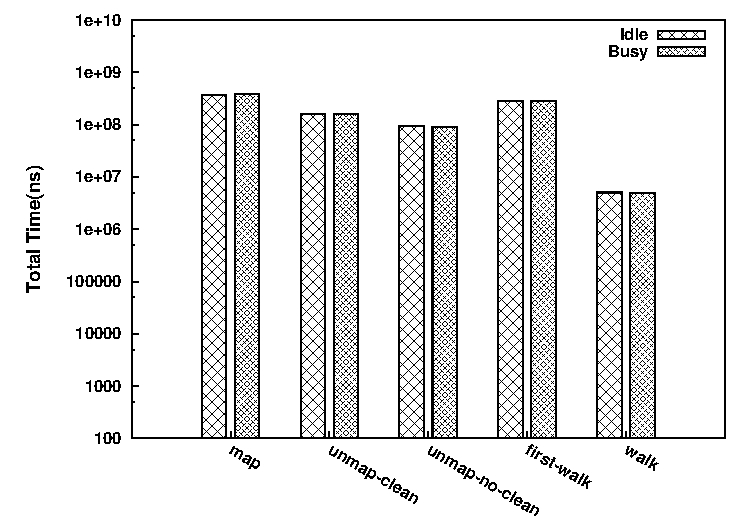
\includegraphics[width=0.9\linewidth]{../figures/alloc}
\label{fig:alloc}
\caption{The different part of allocation time. \emph{map} means the entire time
including the mapping, walking, and unmapping. \emph{unmap} has two options, to
zero out the page (suffixed with "-clean"), and don't do extra things (suffixed
with "-no-clean"). The first walk means the duration of the first time we visit
the allocated space, and walk means the time to do memory walk after we have
touched all the pages several times.}
\end{figure}
To address questions we mentioned, I measured several parts of the overhead in 
figure~\ref{fig:alloc}:
\begin{itemize}
\item total overhead (tagged as "map-full"). Including mapping, memory walking
and unmapping time.
\item first time walk overhead. This will ensure the pages be allocated.
\item unmapping overhead, with/without reset routine. Measuring this part is
for the sake to explore if operating systems can do zero out at reclaim time.
\item regular memory walk after all the pages are assured to exist in memory(I
monitored the swap space used, and it's not grown at any experiment time).
\end{itemize}
These experiments are done under memory idle period, and memory pressure
period. To compare the zero-out strategy, we also measured the allocation
time when memory is scarse resource. In this scenario, the free memory I leave
to operating system is less than 1.5GB, and the allocation unit I used is
1GB, to make sure few free pages are in the system, and it must zero out pages
at the time of granting or revoking them to users.

From figure~\ref{fig:alloc} we can easily find out the allocation is on demand, since regular
walking is much too cheap comparing with the first time memory walk after
mapping a set of memory. And also the performance retains regardless of the
memory pressure. According to that fact, it is only reasonable to zero out
pages on allocation and deallocation time. But the measurement of unmapping
time did not show much information, since the unmapping time is sufficiently
large that we can not distinguish that if it actually does page zero out.

\subsubsection{Benefit from On-Demand Allocation}

\begin{figure}[htb]
\centering
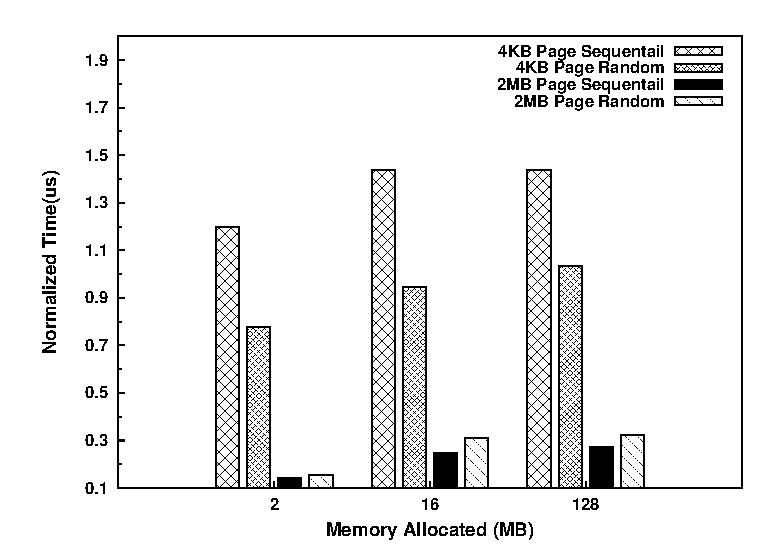
\includegraphics[width=0.8\linewidth]{../figures/on_demand_4k}
\label{fig:on-demand}
\caption{The different of doing random walk and sequential walk through the 
newly allocated 128MB memory. For small page space, random walk would not bring
in the page not needed, thus performs better than sequential walk. But for
large page space, random walk is slower.}
\end{figure}

The on demand allocation is an optmization for virtual memory. To see its
effect, I compared the cost to do random walking and sequential memory walk
on the 128MB newly allocated memory. For space limitation, I only present the
result on 4Byte stride as in figure~\ref{fig:on-demand}. Further results are
uploaded to~\cite{github}, it is consistent with my conclusions here.

Figure~\ref{fig:on-demand} exhibits interesting result: random walk runs
faster with small pages, but slower with large page. In the former case,
don't not bring in unnecessary pages save time, while in later one there
is no much pages to bring in, and poor locality slows it down.

\subsection{Discussion}
One thing hard to illustrate is whether operating system will 'smartly'
allocate some pages for small requests. For example, when user requests for
only 1 page, then allocate the page immediately to avoid a page fault can be
somewhat a good choice. This period is too small to measure correctly just by
using wall clock. However, if the operating system can provide a page fault
counter for each process, then it is still possible to measure such behavior.
Due to both the time limit and space limit, I didn't implement this as part of
the benchmark.
